\documentclass{beamer}
\usepackage[utf8]{inputenc}

\usetheme{Madrid}
\usecolortheme{default}
\usepackage{amsmath,amssymb,amsfonts,amsthm}
\usepackage{tkz-euclide}
\usepackage{listings}
\usepackage{adjustbox}
\usepackage{array}
\usepackage{tabularx}
\usepackage{gvv}
\usepackage{lmodern}
\usepackage{circuitikz}
\usepackage{tikz}
\usepackage{graphicx}

\setbeamertemplate{page number in head/foot}[totalframenumber]

\usepackage{tcolorbox}
\tcbuselibrary{minted,breakable,xparse,skins}



\definecolor{bg}{gray}{0.95}
\DeclareTCBListing{mintedbox}{O{}m!O{}}{%
  breakable=true,
  listing engine=minted,
  listing only,
  minted language=#2,
  minted style=default,
  minted options={%
    linenos,
    gobble=0,
    breaklines=true,
    breakafter=,,
    fontsize=\small,
    numbersep=8pt,
    #1},
  boxsep=0pt,
  left skip=0pt,
  right skip=0pt,
  left=25pt,
  right=0pt,
  top=3pt,
  bottom=3pt,
  arc=5pt,
  leftrule=0pt,
  rightrule=0pt,
  bottomrule=2pt,
  toprule=2pt,
  colback=bg,
  colframe=orange!70,
  enhanced,
  overlay={%
    \begin{tcbclipinterior}
    \fill[orange!20!white] (frame.south west) rectangle ([xshift=20pt]frame.north west);
    \end{tcbclipinterior}},
  #3,
}
\lstset{
    language=C,
    basicstyle=\ttfamily\small,
    keywordstyle=\color{blue},
    stringstyle=\color{orange},
    commentstyle=\color{green!60!black},
    numbers=left,
    numberstyle=\tiny\color{gray},
    breaklines=true,
    showstringspaces=false,
}
\usepackage[utf8]{inputenc}
\usepackage[T1]{fontenc}



%------------------------------------------------------------
%This block of code defines the information to appear in the
%Title page
\title %optional
{2.6.11}
\date{september 29,2025}
%\subtitle{A short story}

\author % (optional)
{Megha Shyam-AI25BTECH11005}
\begin{document}
\begin{frame}{Question}
   Let $\vec a = 4\hat\imath+5\hat\jmath-\hat k$, $\vec b=\hat\imath-4\hat\jmath+5\hat k$, $\vec c=3\hat\imath+\hat\jmath-\hat k$.  
Find $\vec d$ perpendicular to both $\vec b$ and $\vec c$ and satisfying $\vec d\cdot\vec a=21$. 
\end{frame}
\begin{frame}{Theoritical solution}
    Write vectors as column matrices:
\[
\vec a=\begin{pmatrix}4\\5\\-1\end{pmatrix},\quad
\vec b=\begin{pmatrix}1\\-4\\5\end{pmatrix},\quad
\vec c=\begin{pmatrix}3\\1\\-1\end{pmatrix}.
\]

Since $\vec d$ is perpendicular to both $\vec b$ and $\vec c$,  
\[
\vec d = \lambda(\vec b\times \vec c).
\]

Compute the cross product:
\[
\vec b\times \vec c =\begin{pmatrix}
(-4)(-1)-5(1)\\[6pt]
-\big(1(-1)-5(3)\big)\\[6pt]
1(1)-(-4)(3)
\end{pmatrix}
=
\begin{pmatrix}-1\\16\\13\end{pmatrix}.
\]

Thus
\[
\vec d = \lambda \begin{pmatrix}-1\\16\\13\end{pmatrix}.
\]
\end{frame}
\begin{frame}{theoritical solution}
    Now apply the condition $\vec d\cdot \vec a = 21$:
\[
\vec d \cdot \vec a 
= \lambda \begin{pmatrix}-1 & 16 & 13\end{pmatrix}
\begin{pmatrix}4\\5\\-1\end{pmatrix}.
\]

\[
= \lambda(-4+80-13)=\lambda(63).
\]

So
\[
\lambda(63)=21 \quad\Rightarrow\quad \lambda=\tfrac{1}{3}.
\]

Hence
\[
\vec d = \tfrac{1}{3}\begin{pmatrix}-1\\16\\13\end{pmatrix}
= -\tfrac{1}{3}\hat\imath + \tfrac{16}{3}\hat\jmath + \tfrac{13}{3}\hat k.
\]

\[
\boxed{\vec d = -\tfrac{1}{3}\hat\imath + \tfrac{16}{3}\hat\jmath + \tfrac{13}{3}\hat k}
\]
\end{frame}
\begin{frame}[fragile]{C code}
\begin{lstlisting}[language=C]
#include <stdio.h>
// Function to compute cross product
void crossProduct(int a[3], int b[3], int c[3], int K) {
    c[0] = K * (a[1]*b[2] - a[2]*b[1]);  // i component
    c[1] = K * (a[2]*b[0] - a[0]*b[2]);  // j component
    c[2] = K * (a[0]*b[1] - a[1]*b[0]);  // k component
}int  main() {
    int a[3], b[3], c[3], K;
  // Input vectors a and b
    printf("Enter vector a (ax ay az): ");
    scanf("%d %d %d", &a[0], &a[1], &a[2]);
printf("Enter vector b (bx by bz): ");
    scanf("%d %d %d", &b[0], &b[1], &b[2]);
  printf("Enter scalar K: ");
    scanf("%d", &K);
// Compute c = K(a *b)
    crossProduct(a, b, c, K);
  // Print result
    printf("Vector c = %di + %dj + %dk\n", c[0], c[1], c[2]);
return 0;
}




\end{lstlisting}
\end{frame}
\begin{frame}[fragile]

\frametitle{\textbf{Python Plotting Code - Part 1}}
\begin{lstlisting}[language=Python]
import numpy as np
import matplotlib.pyplot as plt
from mpl_toolkits.mplot3d import Axes3D
# Define the vectors
a = np.array([4, 5, -1])
b = np.array([1, -4, 5])
c = np.array([3, 1, -1])
# Find a direction for d (perpendicular to both c and b)
d_dir = np.cross(c, b)
# Find k such that d*a = 21
k = 21 / np.dot(d_dir, a)
d = k * d_dir
# Origin for all vectors
origin = np.zeros(3)
# Set up 3D plot
fig = plt.figure(figsize=(7, 7))
ax = fig.add_subplot(111, projection='3d')



\end{lstlisting}
\end{frame}
\begin{frame}[fragile]
\frametitle{\textbf{Python plotting code - part 2}}
\begin{lstlisting}[language = Python]
ax.quiver(*origin, *a, color='r', label='a', length=np.linalg.norm(a), arrow_length_ratio=0.1)
ax.quiver(*origin, *b, color='g', label='b', length=np.linalg.norm(b), arrow_length_ratio=0.1)
ax.quiver(*origin, *c, color='b', label='c', length=np.linalg.norm(c), arrow_length_ratio=0.1)
ax.quiver(*origin, *d, color='k', label='d', length=np.linalg.norm(d), arrow_length_ratio=0.15)
# Styling and labels
ax.set_xlim([0, 8])
ax.set_ylim([0, 8])
ax.set_zlim([-2, 8])
ax.set_xlabel('X')
ax.set_ylabel('Y')
ax.set_zlabel('Z')
ax.set_title('3D Plot of Vectors a, b, c, and d')
ax.legend()
plt.tight_layout()
plt.show() 
\end{lstlisting}
\end{frame}
\begin{figure}
    \centering
    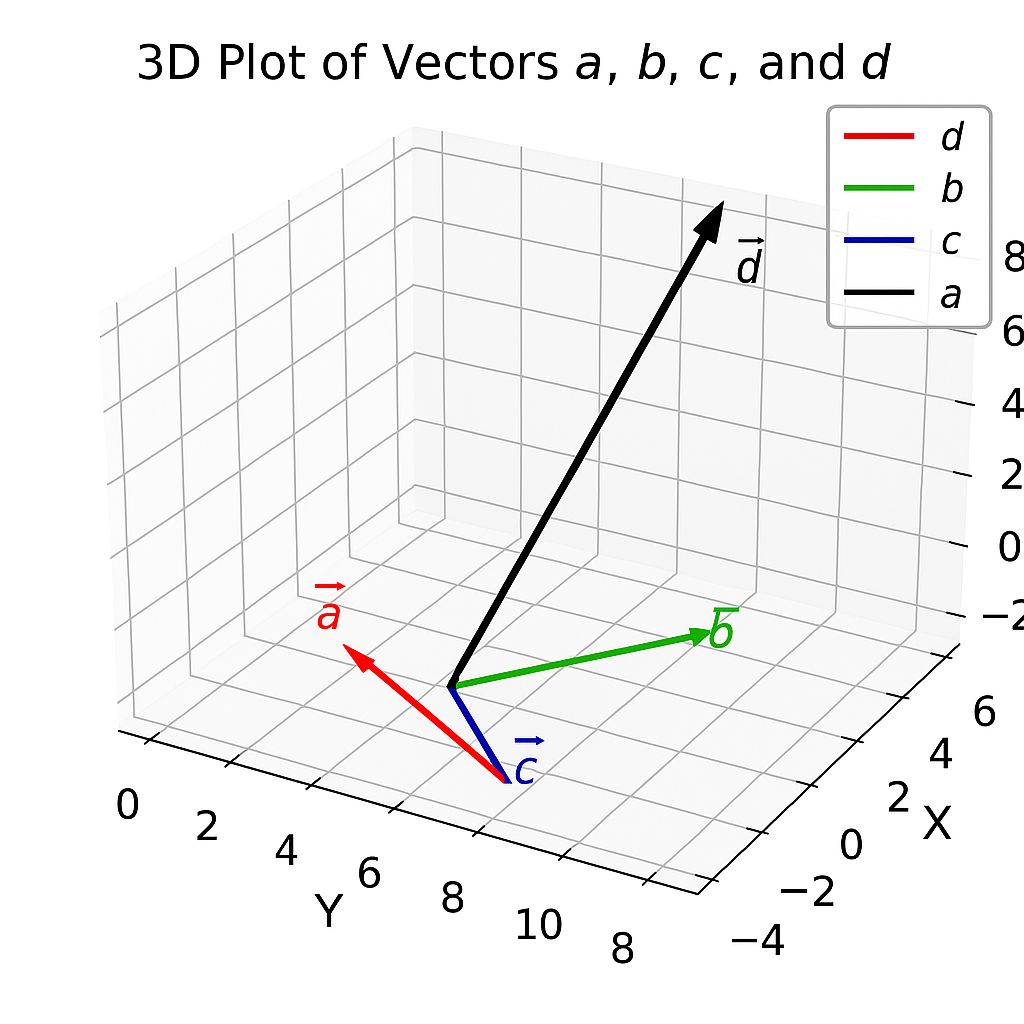
\includegraphics[width=0.5\linewidth]{figs/plot.png}
    \caption{plot}
    \label{fig:placeholder}
\end{figure}
\end{document}